\chapter{Experiment}

Experimentom v našej práci je určovanie hĺbky pamäte a vyhodnotenie vplyvu rôznych
hyper parametrov a typov kontextov na hĺbku pamäte rekurentných SOM.
Cieľom nášho experimentu je aj nájdenie 
optimálnej kombinácie parametrov pre všetky typy porovnávaných sietí a ich vzájomné porovnanie.

\section{Výber konkrétnych trénovacích množín pre experiment}
Trénovacie množiny sme sa snažili zvoliť
takým spôsobom aby sme na nich vedeli otestovať rôzne vlastnosti rekurentných sietí.

Pre náš experiment sme vybrali 3 trénovacie množiny.
Hlavnou trénovaciou množinou, ktorú používame v našom experimente je náhodne generovaná 
sekvencia dlhá 1000 znakov, ktorá pozostáva z písmen $abcd$.
Táto sekvencia obsahuje dostatočné množstvo regularít a malé množstvo unikátnych znakov a teda
aj siete s relatívne malým počtom neurónov sa na nej vedia dobre natrénovať.
Používame ju pri hľadaní optimálných parametrov pre jednotlivé typy sietí.

Ako druhú trénovaciu množinu sme zvolili sekvenciu dlhú 1000 znakov, pričom znaky sú generované
špeciálnym pravdepodobnostným stavovým automatom (Reberov automat). Automat generuje znaky z množiny znakov $ptvxse$.
Táto sekvencia je pre SOMky ťažšia na naučenie a používame ju na overenie toho, či sú siete schopné natrénovať sa aj
na zložitejších nenáhodných sekvenciách. Pri SRN je použitie tejto trénovacej množiny zaujímavejšie,
vďaka vlastnostiam, ktoré SRN má.

Tretí dataset je úryvok z korpusu anglického textu.
Keďže ide o reálny zmysluplný text, nie je to úplne náhodná postupnosť znakov, ale obsahuje určité vzory a opakovania, ktoré by siete mohli vedieť zachytiť
vo svojej vnútorenej reprezentácii.
Tento dataset používame čisto iba na overenie, či 
sú SOMky schopné zachytiť vzory aj v prirodzenom jazyku a teda či sú použiteľné aj pre 
reálne dáta.

\section{Hľadanie optimálnych parametrov sietí}
Na to aby sme mohli porovnať hĺbku pamäte rôznych typov sietí museli sme najskôr
nájsť kombináciu parametrov pri ktorých daný typ siete dosahuje najnižšiu kvantizačnú chybu a 
najvyššie hodnoty pamäťových hĺbok. 

Pri trénovaní samoorganizujúcich sa máp môžeme meniť a optimalizovať veľké množstvo parametrov. 

Ako prvé sme museli správne nastaviť veľkosť okolia víťazného neurónu.
Veľkosť okolia by nemala byť počas trénovania konštantná, ale mala by sa postupne zmenšovať.
Vo fáze doľaďovania by mala byť čo najmenšia.
Excitáciu neurónu v určitom kroku trénovania určuje excitačná funkcia. Zvolili sme spojitú
excitačnú funkciu so spojitým gausovským okolím. 
\begin{equation}
    N(i^{*}, i) = \exp^{- \frac{d^{2}_{E}(i^{*}, i)}{\lambda^{2}(t)}}
\end{equation}
Najvyššiu hodnotu má excitačná funkcia pre víťazný neurón, hodnota excitačnej funkcie pre ostatné 
neuróny v sieti závisí od ich euklidovskej vzdialenosti v mriežke neurónov od ich víťaza. Veľmi vzdialené neuróny 
majú takmer nulovú excitáciu a updatujú svoje váhy minimálne.
Dôležitý je parameter $\lambda$, ktorým znižujem veľkosť okolia postupne v jednotlivých epochách.
Najlepšie výsledky (najnižšie hodnoty kvantizačnej chyby) sme dosiahli pri použití nasledujúceho vzťahu pre výpočet hodnoty tohto parametra
v jednotlivých epochách:
\begin{equation}
    \lambda{(t)} = \lambda_{i} \cdot (\lambda_{f} /\ \lambda_{i})^{t /\ t_{max}}
\end{equation}
Kde $\lambda_{f}$ je konštanta, ktorá určuje rýchlosť klesania. 
$\lambda_{i}$ je polovica maximálnej vzdialenosti dvoch neurónov v mape, resp. 
vzdialenosť dvoch neurónov na koncoch diagonály mriežky neurónov.
$t$ je číslo aktuálnej epochy trénovania. Parametrer $t_{max}$ je celkový počet 
epôch trénovania.


\subsection{Parametre pre RecSOM}
Pri RecSOM kontext tvorí vektor aktivít neurónov z predchádzajúceho kroku.
Aktivita neurónu $y$ je určená vzťahom:

\begin{equation}
    y_{i} = \exp{(-d_{i})}
\end{equation}

Neobsahuje žiadny meniteľný parameter. Hodnota $d_{i}$ je súčet vzdialenosti vstupného vektora od váhového vektora a kontextového vektora od 
kontextového vektora. So zmenšujúcou sa vzdialenosťou excitácia neurónu rastie exponenciálne, čo 
znamená, že víťaz a susedné neuróny budú mať najvyššiu excitáciu a vzdialené neuróny budú mať malú excitáciu.
Výpočet kontextu pri RecSOM nevieme ovplyvnovať žiadnym parametrom.

Môžeme však meniť parameter $\alpha$, ktorý sa používa pri samotnom výpočte vzdialenosti
vstupu od váhového vektora a kontextu od vkontextového vektora. Tento parameter určuje váhu aktuálneho vstupu a váhu kontextu
vo výslednej vzdialenosti.
\begin{equation}
	d_i = (1 - \alpha) \cdot ||x(t) - w_i||^{2} + \alpha \cdot ||y(t-1) - c_i||^{2} \quad c \in R^{N}
\end{equation}
V našich experimentoch sme testovali všetky hodnoty parametra $\alpha$ z uzavretého intervalu
$<0, 1>$ s krokom $0.01$ (dokopy 100 experimentov).

% TODO tabulka, konkrtetne pouzite parametre, vysledky

Výsledky: \\

% výsledky experimentu
\subsection{Activity RecSOM parametre}
Pri modifikovanej verzii RecSOM v ktorej počítame aktivitu neurónov
odlišným spôsobom máme tiež $\beta$ parameter. 
Na výpočet aktivity neurónu používame gaussovskú funkciu, ktorej priebeh ovplyvňujeme
pomocou $\beta$ parametra. To znamená, už to nie je exponenciálna funkcia, ale má odlišný priebeh, 
čo ovplyvňuje výsledné hodnoty aktivácii jednotlivých neurónov. Navyše výslednú hodnotu normalizujeme na
hodnoty z intervalu $<0, 1>$.
\begin{equation}
    \exp^{-\beta \cdot d^2}
\end{equation}

V experimente sme skúšali všetky kombinácie parametrov $\alpha$ a $\beta$.


\subsection{MSOM parametre}
Pri mSOM máme okrem $\alpha$ parametra aj $\beta$ parameter, ktorý určuje váhu
váhového vektora víťaza z predchádzajúceho kroku $w_{i^{*}}$ a váhu kontextu
z predchádzajúceho kroku $y_{i^{*}}$.
V našom experimente skúšame všetky kombinácie $\alpha$ a $\beta$ parametrov.
Hodnoty pre oba parametre sú z uzavretého intervalu $<0, 1>$ s krokom $0.1$ (100 experimentov).


\subsection{Decaying MSOM parametre}
Pri modifikovanej verzii mSOM máme, podobne ako pri mSOM, $\beta$ parameter, ktorý vo vzťahu 
pre výpočet kontextu určuje váhy jednotlivých minulých vstupov. Čím vyššia je hodnota $\beta$
parametra tým vyššiu váhu majú jednotlivé minulé vstupy.
Opäť skúšame všetky kombinácie $\alpha$ a $\beta$ parametrov.
Hodnoty pre oba parametre sú, podobne ako pri mSOM, z uzavretého intervalu $<0, 1>$ s krokom $0.1$

% vysledky



Experimentami sme zistili, že na hĺbku pamäte siete majú vplyv iba niektoré z nich. 
Najdôležitejšie parameters, ktoré vplývajú na hĺbku pamäte neurónovej siete sú parameters $\alpha$ a $\beta$
vo vzťahu pre výpočet vzdialenosti vstupného vektora od určitého neurónu v siete (čiže od jeho váhového a kontextového vektora).
% TODO pridat rovnicu na ilustraciu
Tieto dva parameters určujú pomer dôležitosti aktuálneho vstupu a dôležitosť kontextu, pri výpočte vzdialenosti (kvantizačnej chyby).

Experiment prebiehal nasledujúcim spôsobom:
\begin{itemize}
    \item Vybrali sme vhodnú trénovaciu sekvenciu, počet epôch trénovania a dostatočnú veľkosť pamäťového okna
    \item Spustili sme trénovanie na všetkých kombináciach týchto dvoch parametrov s krokom 0.1
    \item Hodnoty pamäťovej hĺbky sme ukladali do súboru
    \item Na záver sme vykreslili heatmapu, ktorá znázorňuje aká bola pamäťová hĺbka pre rôzne kombinácie parametrov.
\end{itemize}

% TODO vyber rychlosti ucenia (konstantna / postupne zmensujuca?)

Počet epôch sme určili na základe kvantizačnej chyby.
Počet epôch sme postupne zvyšovali a keď kvantizačná chyba prestala signifikantne klesať, resp. dosiahla 
svoje minimum zastavali sme ho na tejto hodnote a ďalej nezvyšovali. SOM sa dokážu relatívne rýchlo učiť a 
teda počet epôch nemusí byť vysoký, čo je veľkou výhodou pri experimentovaní, kedže trénovanie netrvá príliš dlhú dobu
a tým pádom sme mohli vyskúšať viac kombinácii a modifikácii.

Dostatočnú veľkosť pamäťového okna sme určili podobne ako počet epôch. Parameter sme postupne zvyšovali
a zastavili na hodnote, keď pamäťová hĺbka siete prestala stúpať, čiže veľkosť pamäťového okna už
neovplyvňovala hĺbku pamäte a ďalšie zvyšovanie parametra nemalo zmysel. 

Na základe tohto sme zistili, že pre každý typ siete sú ideálne hodnoty týchto parametrov odlišné.


\section{Vyhodnotenie rôznych kombinácii alpha a beta parametrov}

The table \ref{table:1} is an example of referenced \LaTeX elements.
 
\begin{table}[h!]
\centering
\begin{tabular}{|c|c|} 
 \hline
 Parameter & Hodnota \\ 
 \hline\hline
 1 & 6  \\ 
 \hline
 2 & 7   \\
 \hline
 3 & 545  \\
 \hline
 4 & 545  \\
 \hline
 5 & 88 \\  
 \hline
\end{tabular}
\caption{Parametre RecSOM siete}
\label{table:1}
\end{table}


\begin{figure}[H]
    \centering
    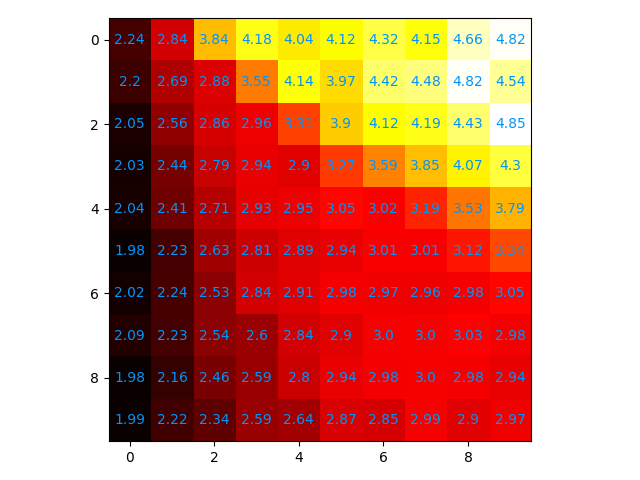
\includegraphics[width=8cm]{assets/recsom_abcd}
    \caption{Rec SOM results}
\end{figure}


\begin{table}[h!]
    \centering
    \begin{tabular}{|c|c|} 
     \hline
     Parameter & Hodnota \\ 
     \hline\hline
     1 & 6  \\ 
     \hline
     2 & 7   \\
     \hline
     3 & 545  \\
     \hline
     4 & 545  \\
     \hline
     5 & 88 \\  
     \hline
    \end{tabular}
    \caption{Parametre mSOM siete}
    \label{table:2}
\end{table}

\begin{figure}[H]
    \centering
    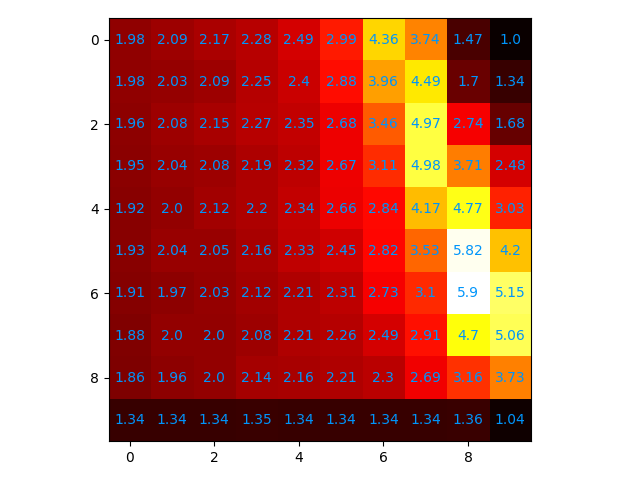
\includegraphics[width=8cm]{assets/msom_abcd}
    \caption{MSOM results}
\end{figure}


\begin{table}[h!]
    \centering
    \begin{tabular}{|c|c|} 
     \hline
     Parameter & Hodnota \\ 
     \hline\hline
     1 & 6  \\ 
     \hline
     2 & 7   \\
     \hline
     3 & 545  \\
     \hline
     4 & 545  \\
     \hline
     5 & 88 \\  
     \hline
    \end{tabular}
    \caption{Parametre leaky mSOM siete}
    \label{table:2}
\end{table}

\begin{figure}[H]
    \centering
    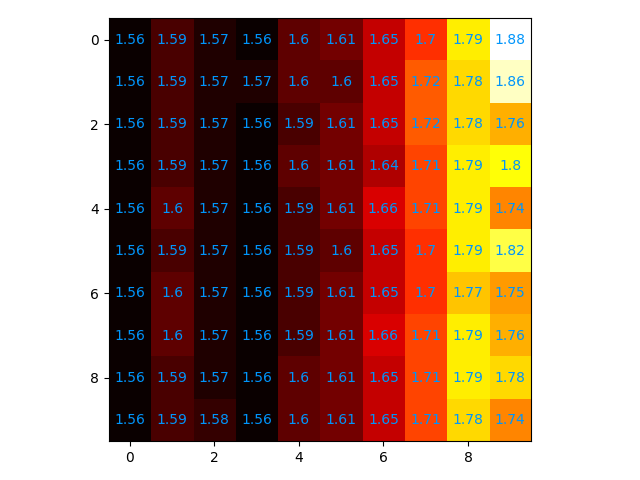
\includegraphics[width=8cm]{assets/leakymsom_abcd}
    \caption{Leaky MSOM results}
\end{figure}


\section{Experiment so SRN a Reberovým automatom}



